\documentclass{article}
\usepackage{amsmath, amsthm, amssymb, amsfonts, bm}
\usepackage{graphicx}
\usepackage[T1]{fontenc}
\usepackage[utf8]{inputenc}
\usepackage[a4paper]{geometry}
\usepackage{fancyhdr}
\usepackage[algo2e]{algorithm2e}
\fontfamily{cmr}

\title{DD2424 - Assignment 3 (bonus)}
\author{Oskar Stigland \\ stigland@kth.se}

\pagestyle{fancy}
\fancyhf{}
\rhead{stigland@kth.se}
\lhead{DD2424 - Deep Learning in Data Science}
\rfoot{Page \thepage}

\begin{document}
%\maketitle

	\begin{titlepage}
		\begin{center} 
			
			\rule{\linewidth}{0.5mm}\\[0.5 cm]
			{ \huge \bfseries DD2424 - Assignment 3 (bonus)}\\[0.3 cm] % Title of your document
			\rule{\linewidth}{0.5mm}\\[1 cm]
					
			\small\vfill
			\begin{center}
			\centering
			{\large \bfseries \textsc{Summary}}\\
			\vspace{1cm}
			\begin{minipage}{10cm}
				
				For this extension,  I have explored \texttt{batch normalization} further, looking at \texttt{precise batch normaliztion} and \texttt{adaptive batch normalization}. The improvements seem to be marginal. Then, I have also attempted to increase the efficiency and performance when training a deep network,  specifically testing variants of a network with $7$ hidden layers - one similar to that in the assignment, as well as a deeper variants with more hidden units. I have attempted to train these networks with a cyclical learning rate as well as attempting to gauge the improvements of instead using \texttt{Adam} and \texttt{AdaGrad}.\\\\
%
	The code for the assignment has been written in \texttt{python}. I have implemented the neural network as a class. For the hand-in, all of the code has been put toghether in a main file with all the functions and the class declared at the top. For the hand-in, I have also commented out the saving of generated figures and results in JSON files, as well as omitting some of the case-specific testing and gradient testing.
			\end{minipage}
			\end{center}
			\large\vfill
						

		\end{center}	
		
		\begin{minipage}{0.4\textwidth}
			\begin{flushleft} \large
				%\emph{Student:}\\
				Oskar \textsc{Stigland}\\
				DD2424\\
				Spring 2023
			\end{flushleft}
		\end{minipage}	

	\end{titlepage}

\newpage

\subsection*{Exploring \texttt{batch normalization} further}
	My initial extension to the third assignment is a further exploration of \texttt{batch normalization}, for which I have looked into so-called precise and \texttt{adaptive batch normalization}, respectively. For all experiments in this first section, I have used a $4$-layer neural network with $100$ units in each layer and $\lambda = 0.01$, with a cyclical learning rate, training for $30$ epochs with $\eta_{min} = 1e-4$, $\eta_{max} = 1e-2$ and \texttt{ns}$=900$.

\subsubsection*{Precise \texttt{batch normalization}}
	For \texttt{precise batch normalization}, I computed the layer-to-layer normalization parameters at for each $20$th batch, such that after e.g. $20$ batches, the parameters would be computed for those $20$ preceding batches, and so on for $100$ batches for each epoch. Then, after each epoch I computed the normalization parameters on the entire training dataset and checked the accuracy on the testing set. The results are provided as a comparison with \texttt{adaptive batch normalization} and vanilla \texttt{batch normalization} in a figure below. The effect seems to be marginal with respect to loss metrics and the testing accuracy. The loss curve is perhaps slightly smoother.

\subsubsection*{Adaptive \texttt{batch normalization}}
	For \texttt{adaptive batch normalization}, I saved the normalization parameters after each epoch and recomputed them on the testing dataset. For this latter part, I also initially used an image flip probability of $p=0.5$ at each epoch when comuting the parameters. Again, the effects are very marginal - perhaps even bordering on indiscernible. To compare the results, I have plotted the training loss and testing accuracies for vanilla \texttt{batch normalization}, \texttt{precise batch normalization}, \texttt{adaptive batch normalization} and a combined approach, with an image flip probability of $p=0.1$. For the exponential moving average, $\alpha=0.8$ is used.
	\begin{figure}[h!]
		\centering
		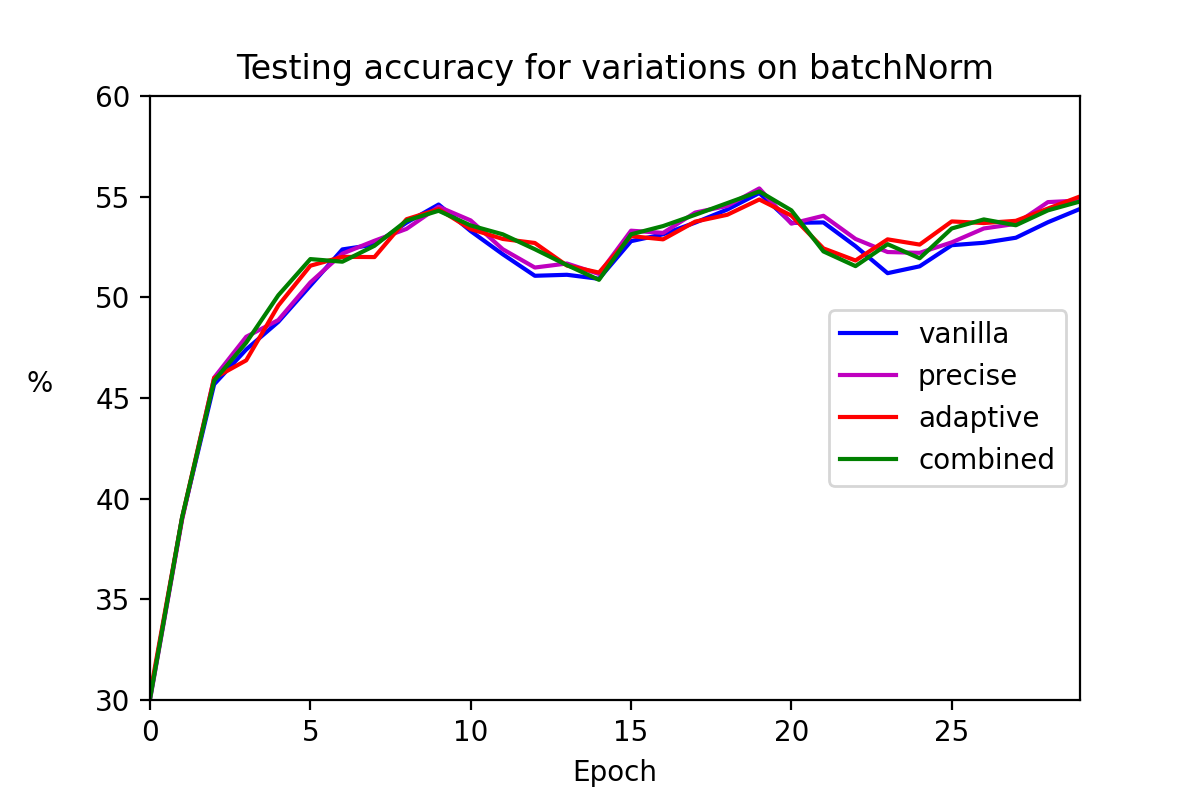
\includegraphics[width=7cm]{../plots/acc_comp_bn.png}
		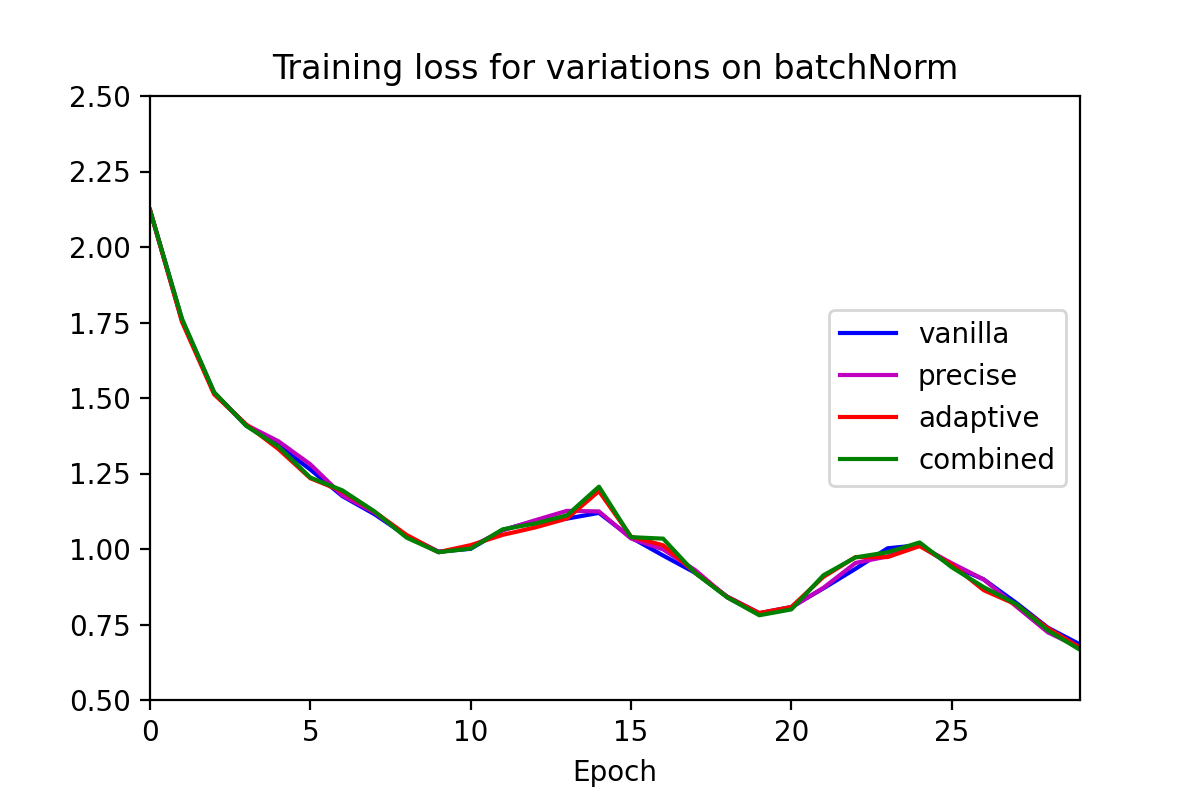
\includegraphics[width=7cm]{../plots/loss_comp_bn.png}	
		\caption{Testing accuracy and training loss for four variations on \texttt{batch normalization}, trained for $30$ epochs with a cyclical learning rate and a $4$-layer network with $100$ nodes in each layer and $\lambda = 0.01$.}
 	\end{figure}\\
	As is evident from the figure, there is no clear improvement for any of the models. The three modifications (precise, adaptive and combined) seem to achieve a slight bump in accuracy towards the end as compared to the vanilla implementation - but it is indeed slight. All models achieve a maximum accuracy of some $\sim55$\%. 

\newpage
\subsection*{Improving training for a deep network}
	To test different optimization paradigms and potentially improve the training process for a deep network, I have ventured into testing \texttt{Adam} with a fixed learning rate and \texttt{AdaGrad} with a decaying learning rate, which decays according to
	$$\eta_n = \eta_0 \times \exp(-\Delta\eta \times t)$$
	where $\delta\eta$ is the decay rate, set to $\Delta\eta = 10^{-4}$, and $\eta_0 = 0.01$. For \texttt{Adam}, we have a fixed $\eta = 0.001$. Further, for this particular experiment, I have chosen to use \texttt{adaptive batch normalization} and for the exponential moving average I use $\alpha = 0.8$. Additionally, I have also employed \texttt{He} initialization in order to improve gradient calculations across the training process, and $\lambda = 0.01$. For the model, I have used $7$ hidden layers with two variations on depth:
	\begin{align*}
		\bm{m}_1 &= [50, 50, 50, 20, 20, 10, 10] \\
		\bm{m}_2 &= [100, 100, 100, 50, 50, 20, 20]
	\end{align*}
	The results for all models are presented in the figures below.
	\begin{figure}[h!]
		\centering
		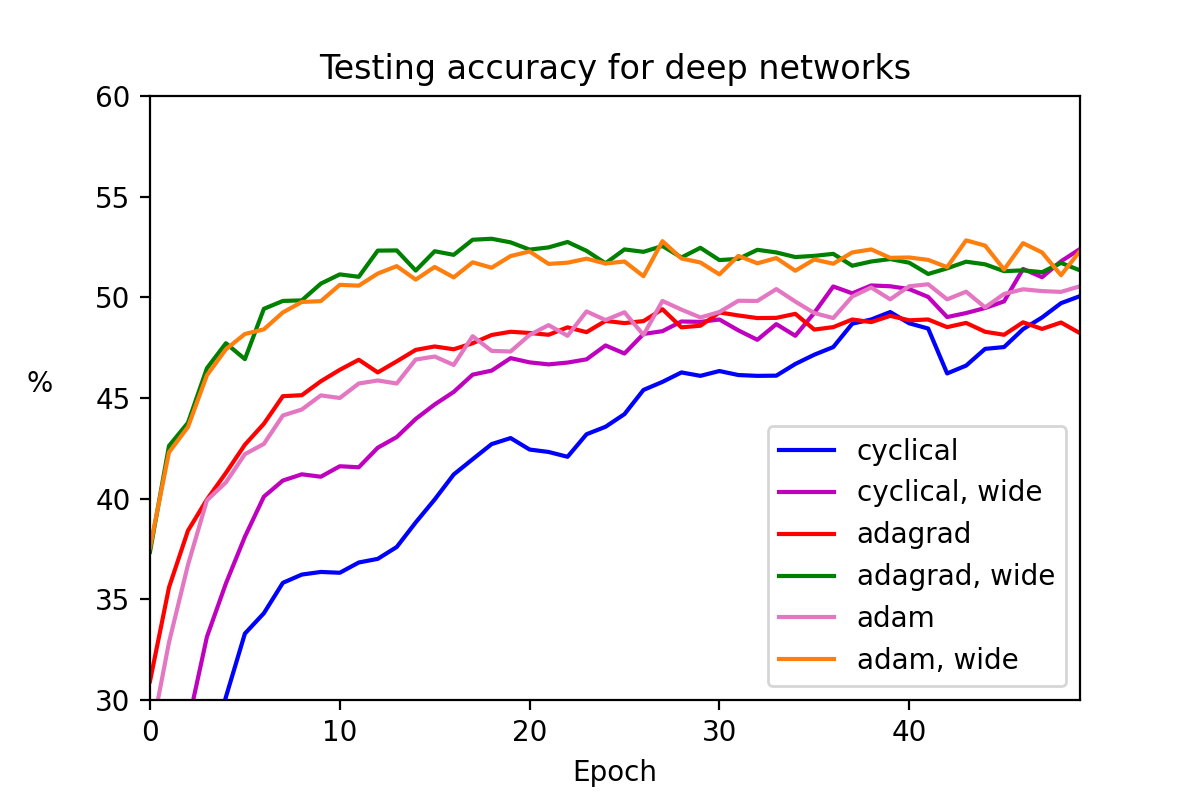
\includegraphics[width=7cm]{../plots/acc_comp_deep.png}
		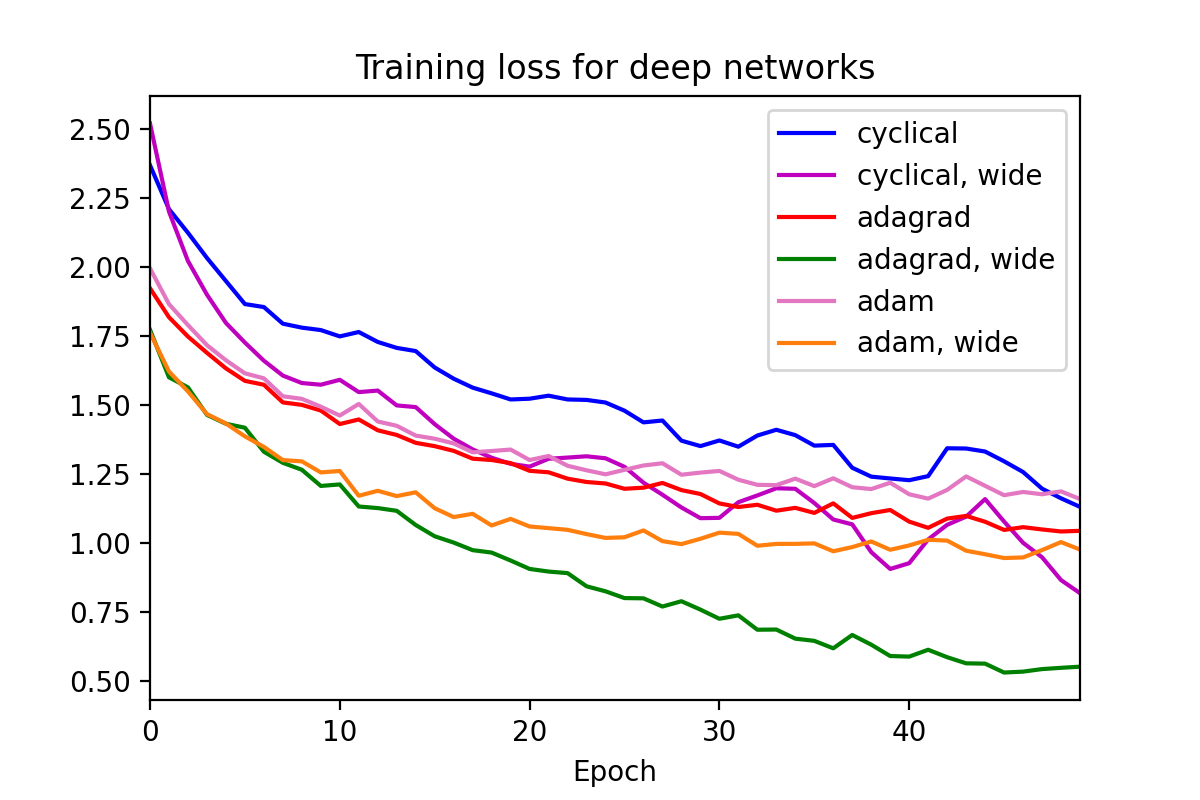
\includegraphics[width=7cm]{../plots/loss_comp_deep.png}	
		\caption{Testing accuracy and training loss for deep networks, trained for $50$ epochs with a cyclical learning rate, \texttt{AdaGrad} or \texttt{Adam}.}
 	\end{figure}\\
	In this particular case, the wide network, i.e. with $\bm{m}_2$ and \texttt{AdaGrad} outperforms the others - including the same network with \texttt{Adam} with respect to the training loss. However, the accuracy is more or less identical for the two cases. Surprisingly, seems also the cyclical learning rate scheme reaches a similar accuracy with $\bm{m}_2$ after $50$ epochs. However, \texttt{AdaGrad} and \texttt{Adam} provide more stable training, which is evident from both the accuracy and loss plots, although the final result is no dramatic improvement over the cyclical learning rate. Looking at the figure, it is evident that hidden layers with more units perform better, and that models train with \texttt{Adam} and \texttt{AdaGrad} converge much faster than when a cyclical learning rate is used. 

\end{document}